\documentclass[a4paper,14pt,oneside,openany]{memoir}

%%% Задаем поля, отступы и межстрочный интервал %%%

\usepackage[left=10mm, right=15mm, top=20mm, bottom=20mm]{geometry} 

\usepackage[english, russian]{babel}    
\usepackage{longtable,ltcaption}                    % Длинные таблицы
\usepackage{multirow,makecell}                      % Улучшенное форматирование таблиц
\usepackage{booktabs}                               % Еще один пакет для красивых таблиц
\usepackage{soulutf8}                               % Поддержка переносоустойчивых подчёркиваний и зачёркиваний
\usepackage{icomma}                                 % Запятая в десятичных дробях
\usepackage{hyphenat}                               % Для красивых переносов
\usepackage{textcomp}                               % Поддержка "сложных" печатных символов типа значков иены, копирайта и т.д.
\usepackage[version=4]{mhchem}                      % Красивые химические уравнения
\usepackage{amsmath} 

\usepackage[utf8]{inputenc}

\usepackage[section]{placeins}
\usepackage{amsthm}
\usepackage{amssymb}
\usepackage{enumerate}
\usepackage{stmaryrd}
\usepackage{cmll}
\usepackage{mathrsfs}
\usepackage{proof}
\usepackage{tikz}
\usepackage{multicol}
\usepackage{mathabx}
\usepackage{pdflscape}
\usepackage{listings}
\usepackage{xcolor}

%opening
\title{}
\author{}

\definecolor{codegreen}{rgb}{0,0.6,0}
\definecolor{codegray}{rgb}{0.5,0.5,0.5}
\definecolor{codepurple}{rgb}{0.58,0,0.82}

\lstdefinestyle{mystyle}{
	keywordstyle=\color{codepurple},
	numberstyle=\tiny\color{codegray},
	stringstyle=\color{codegreen},
	basicstyle=\ttfamily\footnotesize,
	breakatwhitespace=false,         
	breaklines=true,                 
	captionpos=b,                    
	keepspaces=true,                 
	numbers=left,                    
	numbersep=5pt,                  
	showspaces=false,                
	showstringspaces=false,
	showtabs=false,                  
	tabsize=2
}

\lstset{style=mystyle}


\begin{document}

\thispagestyle{empty}

\begin{center}
	
	Национальный исследовательский университет ИТМО\\
	Факультет информационных технологий и программирования\\
	Прикладная матеметика и информатика\\
	
	\vspace{20pt}
	
\end{center}

\vfill

\begin{center}
	\textbf {\fontsize{100}{120}\selectfont Методы оптимизации
	} \\  
	Отчет по лабораторной работе №4
	
\end{center}

\vfill

\begin{flushright}
	
	\hfill {
		Работу \\
		выполняли: \\
		Кольченко Антон М32371 \\ 
		Гайнанов Ильдар М32371 \\ 
		Муфтиев Руслан М32331\\ 
	}
	\vspace{20pt}
	
\end{flushright}

\vfill

\begin{center}
	Санкт-Петербург\\
	2023
\end{center}

\chapter*{Введение}
\textbf{Постановка задачи:}

\begin{enumerate}
\item Изучить использование вариантов SGD (torch.optim) из PyTorch. Исследовать эффективность и сравнить с собственными реализациями из 2 работы.
\item Изучить использование готовых методов оптимизации из SciPy 

(scipy.optimize.minimize, scipy.optimize.least\_squares) 
\begin{enumerate}
\item Исследовать эффективность и сравнить с собственными реализациями из 3 работы.
\item Реализовать использование PyTorch для вычисления градиента и сравнить с другими подходами.
\item Исследовать, как задание границ измерения параметров влияет на работу методов из SciPy.
\end{enumerate}
\item Исследовать использование линейных и нелинейных ограничений при использовании scipy.optimize.minimize из SciPy. Рассмотреть случаи, когда минимум находится на границе заданной области и когда он расположен внутри.
\end{enumerate}

\chapter{Практическая часть}
 
\section{Сравнение реализаций SGD}
\subsection{Сравнение путей реализаций}
\begin{figure}[ht]
	\centering
	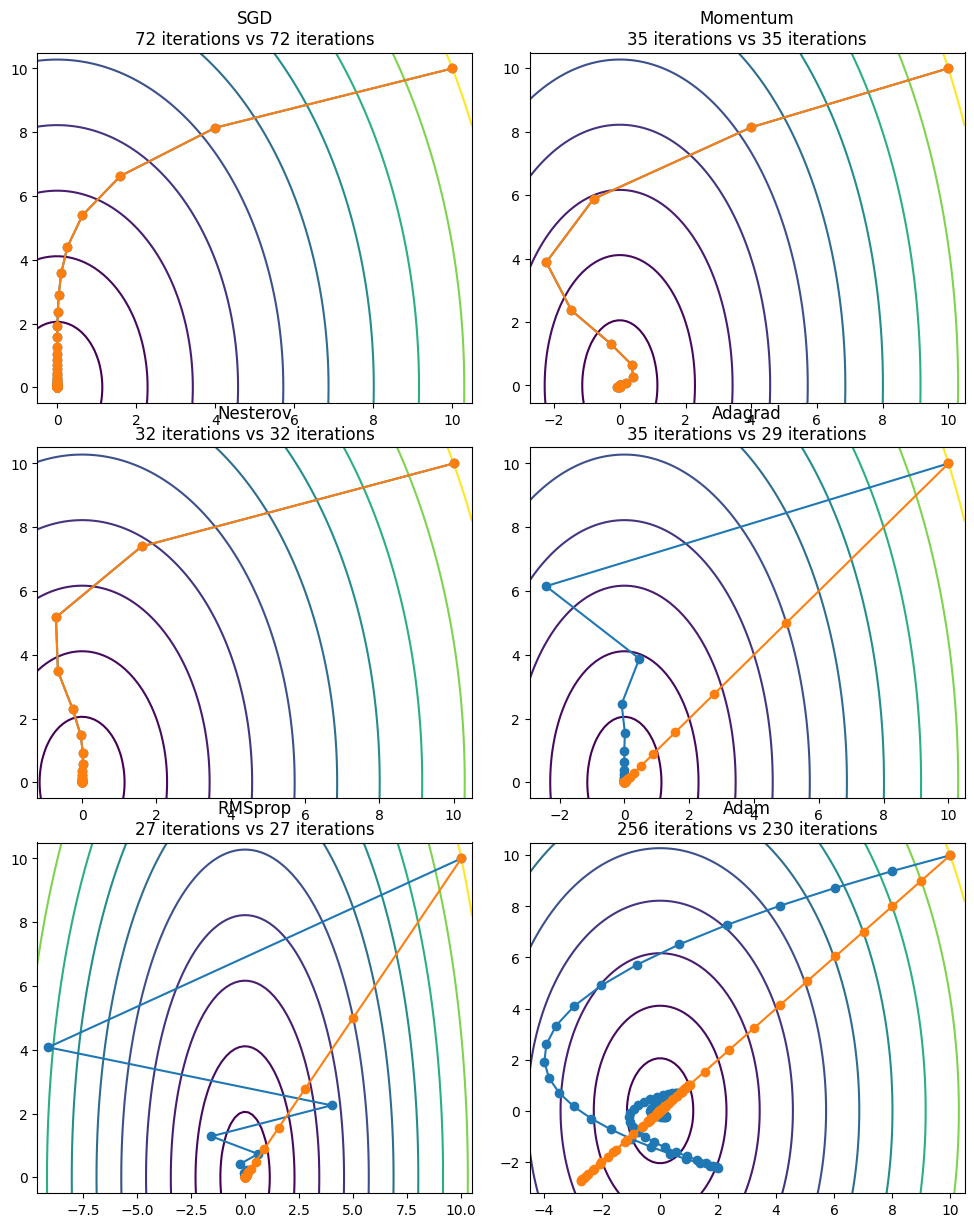
\includegraphics[width=1\textwidth]{img/4_1_1.png}
	\caption{Хорошо обусловленная функция. Синий - наша реализация, оранжевый - реализация из Pytorch}
\end{figure}

\begin{figure}[ht]
	\centering
	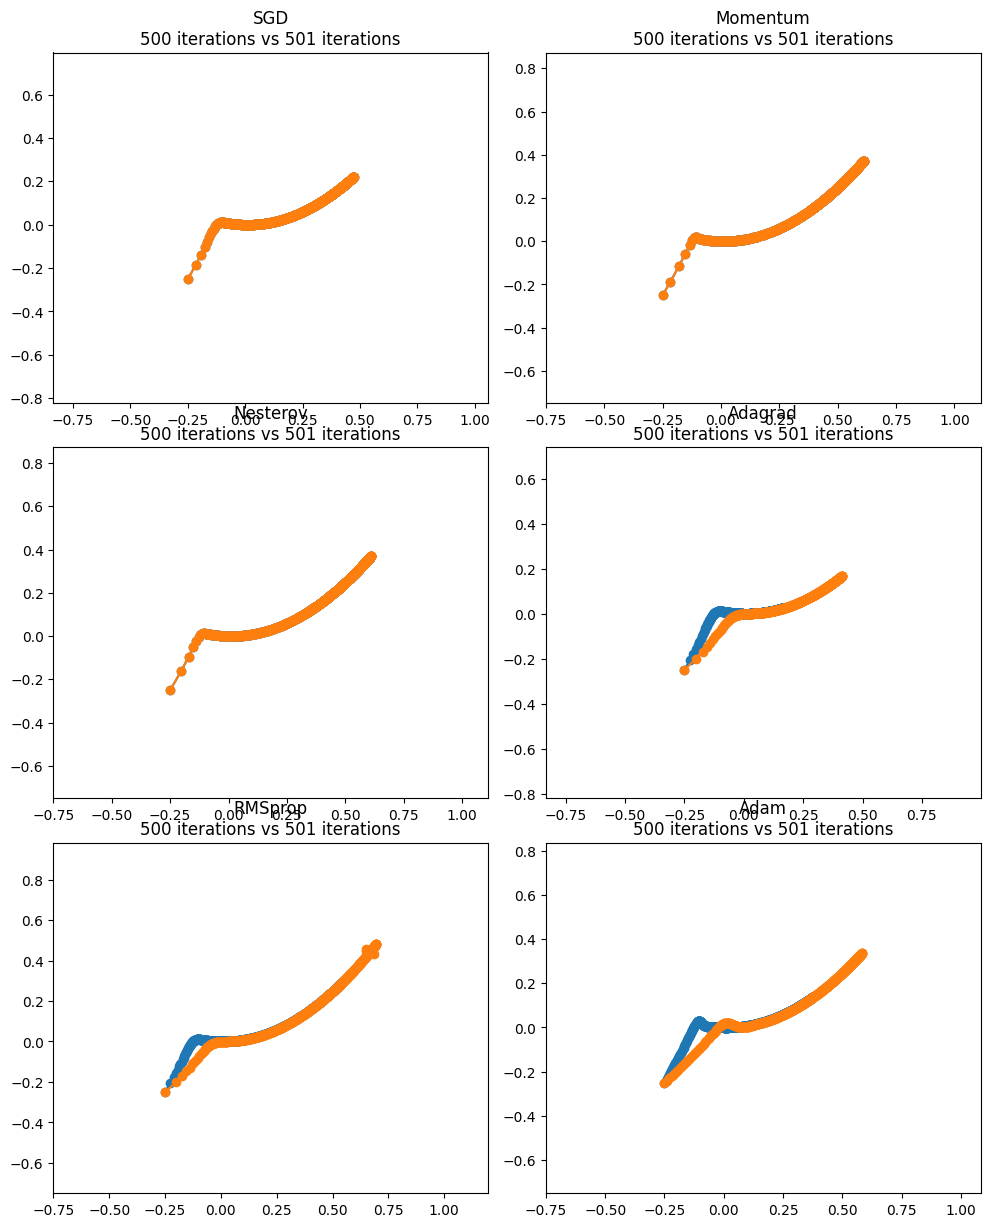
\includegraphics[width=1\textwidth]{img/4_1_2.png}
	\caption{Плохо обусловленная функция - функция Розенброка. Синий - наша реализация, оранжевый - реализация из Pytorch}
\end{figure}
\clearpage
\subsection{Выводы}
\begin{enumerate}
\item Путь реализаций стандартного стохастического градиентного спуска, модификаций Momentum и Nesterov при равных параметрах полностью совпадают. Необходимо будет присмотреться к другим характеристикам методов.
\item Пути остальных алгоритмов не совпадают. Однако, поиграв с параметрами, можно добиться схожих скоростей сходимости. Если посмотреть на реализации методов из PyTorch, можно заметить, что уже первый шаг имеет отличающееся направление. Делаем вывод, что PyTorch в этих методах вычисляет градиент иным способом.
\item Чудес не бывает - несмотря на отличия в пути, ни одна из реализаций алгоритмов не справляется с функцией Розенброка. Для нее все еще нужна смена алгоритма.
\end{enumerate}

\subsection{Сравнение производительности реализаций}
\FloatBarrier
\begin{table}
	\centering
	\begin{tabular}{|c|c|c| }
	\hline
	& time, s & mem usage \\
	\hline
	SGD & 0.44 & 74070 \\
	\hline
	\textbf{PT} SGD & 0.053 & 15611 \\
	\hline
	Momentum & 0.203 & 44648  \\
	\hline
	\textbf{PT} Momentum & 0.026 & 8980  \\
	\hline
	Nesterov & 0.187 & 42526  \\ 
	\hline
	\textbf{PT} Nesterov & 0.025 & 8362  \\ 
	\hline
	AdaGrad & 0.189 & 44333 \\
	\hline
	\textbf{PT} AdaGrad & 0.023 & 8191   \\ 
	\hline
	RMSProp & 0.158 & 37673  \\
	\hline
	\textbf{PT} RMSProp & 0.022 & 7409  \\ 
	\hline
	Adam & 1.458 & 142363  \\
	\hline
	\textbf{PT} Adam & 0.204 & 45147  \\ 
	\hline
	\end{tabular}
	\caption{Таблица расхода ресурсов на использование методов}
\end{table}

\clearpage

\subsection{Выводы}
\begin{enumerate}
\item Неудивительно, что реализации на PyTorch оказались в разы экономнее, чем наши реализации. Наши реализации написаны полностью на Python, который не знаменит высокой производительностью, тогда как методы в PyTorch <<под капотом>> реализованы на C++.
\end{enumerate}
\newpage
	
\section{Сравнение реализаций нелинейной регрессии}
\FloatBarrier
\begin{figure}[ht]
	\centering
	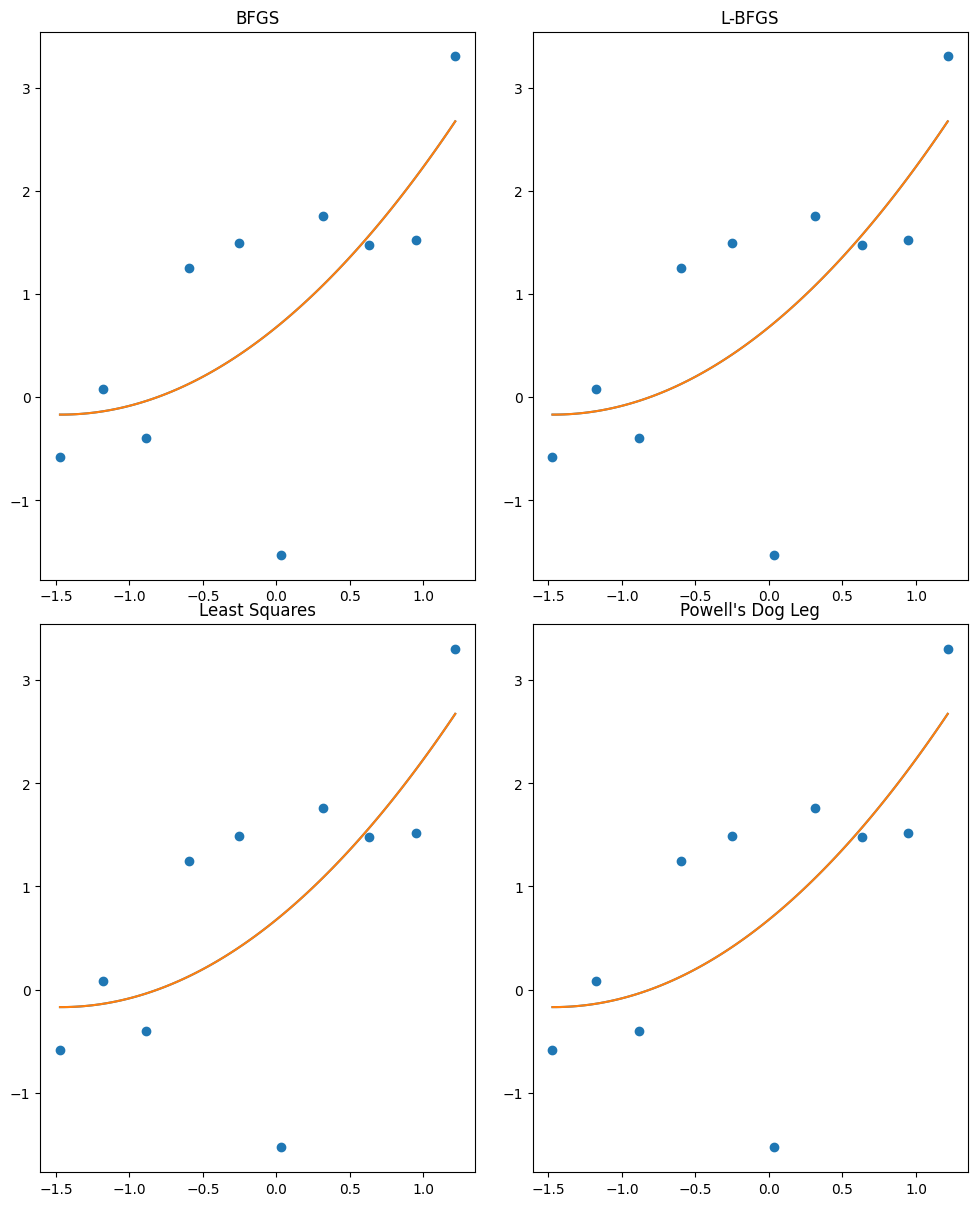
\includegraphics[width=0.9\textwidth]{img/4_2_1.png}
\end{figure}
\FloatBarrier
\begin{table}
	\centering
	\begin{tabular}{|c|c|c| }
	\hline
	& time, s & mem usage \\
	\hline
	BFGS & 1.32 & 270272 \\
	\hline
	\textbf{SP} BFGS & 0.012 & 14357 \\
	\hline
	L-BFGS & 2.238 & 119209 \\
	\hline
	\textbf{SP} L-BFGS & 0.008 & 23017  \\
	\hline
	Gauss-Newton & 0.016 & 104732  \\ 
	\hline
	\textbf{SP} Gauss-Newton & 0.034 & 11512 \\ 
	\hline
	Dog Leg & 0.226 & 156694 \\
	\hline
	\textbf{SP} Dog Leg (dogbox) & 0.032 & 12930   \\ 
	\hline
	\end{tabular}
	\caption{Таблица расхода ресурсов на использование методов}
\end{table}
\FloatBarrier
\subsection{Выводы}
Выводы схожи с пунктом про градиентные спуски.
\begin{enumerate}
\item Наши реализации методов и реализации в SciPy выдают примерно одинаковый результат (разница в миллионные доли, на графике никак не будет видно).
\item Реализации в SciPy работают быстрее (за исключением метода наименьших квадратов) и занимают в разы меньше памяти.
\end{enumerate}
\newpage
\section{Сравнение реализаций градиентов}
Будем вычислять градиент методом двусторонней разности, с помощью библиотеки numdifftools и PyTorch.
\FloatBarrier
\begin{table}
	\centering
	\begin{tabular}{|c|c|c|c| }
	\hline
	& $\Delta_{manual}$ & time, s & mem usage \\
	\hline
	Manual & N/A & 0.00022 & 6632 \\
	\hline
	numdifftools & $3.75*10^{-9}$ & 0.02 & 22304 \\
	\hline
	PyTorch & $3.75*10^{-9}$ & 0.0005 & 1281 \\
	\hline
	\end{tabular}
	\caption{Таблица расхода ресурсов на использование методов}
\end{table}
\FloatBarrier
\subsection{Выводы}
Выводы схожи с пунктом про градиентные спуски.
\begin{enumerate}
\item Удивительно, но ручное вычисление градиента работает быстрее всего...
\item ...но при этом меньше всего памяти расходует вычисление через PyTorch.
\item Вероятно, Torch мог бы быть быстрее, но какое-то время тратится на конверсию np.ndarray -> torch.Tensor -> np.ndarray
\item В целом, вычисление градиента все равно занимает не очень много ресурсов, так что выбор алгоритма не будет кардинально менять время работы.
\end{enumerate}
\newpage
\section{Зависимость результатов минимизации от границ переменной}
Рассматриваем функцию $y = 3 + 3x + 3x^2$, ограничиваем переменную отрезком $[-a, a]$.
\FloatBarrier
\begin{table}
\centering
Gauss-Newton: \\
\begin{tabular}{|c|c|c|c| }
	\hline
	$a$ & $f_{loss}$ & time, s & mem usage \\
	\hline
	1 & 129.6 & 0.05 & 13205 \\
	\hline
	3 & $0.016$ & 0.1 & 13243 \\
	\hline
	5 & $0.013$ & 0.128 & 12844 \\
	\hline
	10 & $0.013$ & 0.1 & 12792 \\
	\hline
	100 & $0.013$ & 0.11 & 12840 \\
	\hline
\end{tabular} \\
Powell's Dog Leg: \\
\begin{tabular}{|c|c|c|c| }
	\hline
	$a$ & $f_{loss}$ & time, s & mem usage \\
	\hline
	1 & 129.6 & 0.012 & 12942 \\
	\hline
	3 & $0.016$ & 0.03 & 12978 \\
	\hline
	5 & $0.013$ & 0.07 & 13177 \\
	\hline
	10 & $0.013$ & 0.08 & 13132 \\
	\hline
	100 & $0.013$ & 0.07 & 13178 \\
	\hline
\end{tabular} \\
\caption{Таблица расхода ресурсов на использование методов}
\end{table}
\FloatBarrier
\subsection{Выводы}
\begin{enumerate}
\item Выбор ограничений не оказывает значимого влияния на расход оперативной памяти.
\item Чем больше ограничение, тем медленнее работает метод - вплоть до какого-то значения. В какой-то момент оно перестает иметь смысл - шаг методов никогда не окажется вне слишком больших ограничений.
\item Однако если сделать ограничение слишком маленьким, то метод остановится до достижения минимума.
\end{enumerate}
\newpage
\section{Зависимость результатов минимизации от границ переменной, линейные / нелинейные ограничения}
\FloatBarrier
\begin{table}
\centering
$x_0 = (-30; 50)$ \\
$f = f_{Rosenbrock}$: \\
\begin{tabular}{|c|c|c|c|c|c| }
	\hline
	$constraint$ & $x$ & itercount & time, s & mem usage & note \\
	\hline
	$\emptyset$ & $\approx min$ & 172 & 0.458 & 14235 & \\
	\hline
	$y \ge 0.5x$ & $(0.054; 0.027)$ & 67 & 0.133 & 18553 & 1 \\
	\hline
	$y \le 2x$ & $\approx min$ & 34 & 0.065 & 18055 & \\
	\hline
	$y \le x$ & $\approx min$ & 36 & 0.083 & 21268 & \\
	\hline
	$y \ge x$ & $(5.55; 30.8)$ & 100 & 0.188 & 18585 & 1 \\
	\hline
	$y = x$ & $\approx min$ & 18 & 0.032 & 20119 & \\
	\hline
	$B((1; 1), 1)$ & $\approx min$ & 37 & 0.107 & 20995 & \\
	\hline
	$B((0; 1), 1)$ & $\approx min$ & 44 & 0.118 & 20552 & \\
	\hline
	$B((0; 0), 1)$ & $(0.79; 0.62)$ & 45 & 0.115 & 24083 & 2 \\
	\hline
	$\overline{B((1; 1), 1)} $ & $(0.43; 0.18)$ & 75 & 0.205 & 20400 & 2 \\
	\hline
	$\overline{B((0; 0), 1)}$ & $(-0.78; 0.62)$ & 37 & 0.18 & 21020 & 1 \\
	\hline
\end{tabular} \\
$f$ - простая функция с точкой минимума $(1, 1)$: \\
\begin{tabular}{|c|c|c|c|c|c| }
	\hline
	$constraint$ & $x$ & itercount & time, s & mem usage & note \\
	\hline
	$\emptyset$ & $\approx min$ & 30 & 0.129 & 14021 & \\
	\hline
	$y \ge 0.5x$ & $\approx min$ & 4 & 0.003 & 18537 & \\
	\hline
	$y \le 2x$ & $\approx min$ & 22 & 0.061 & 18191 & \\
	\hline
	$y \le x$ & $\approx min$ & 15 & 0.03 & 18191 & \\
	\hline
	$y \ge x$ & $\approx min$ & 26 & 0.05 & 18055 &  \\
	\hline
	$y = x$ & $\approx min$ & 19 & 0.04 & 20981 & \\
	\hline
	$B((1; 1), 1)$ & $\approx min$ & 25 & 0.085 & 21050 & \\
	\hline
	$B((0; 1), 1)$ & $\approx min$ & 32 & 0.085 & 20552 & \\
	\hline
	$B((0; 0), 1)$ & $(0.81; 0.59)$ & 23 & 0.057 & 23481 & 2 \\
	\hline
	$\overline{B((1; 1), 1)} $ & $(1.71; 1.71)$ & 20 & 0.058 & 20866 & 2 \\
	\hline
	$\overline{B((0; 0), 1)}$ & $\approx min$ & 25 & 0.061 & 20368 &  \\
	\hline
\end{tabular} \\
\small{1 - минимум лежит в области ограничения, но само ограничение расположено так, что функция не может сойтись}\\
\small{2 - минимум не лежит в области}\\
\caption{Таблица расхода ресурсов на использование методов}
\end{table}
\FloatBarrier
\subsection{Выводы}
\begin{enumerate}
\item Линейные и нелинейные ограничения требуют заметно больше оперативной памяти (но все еще в пределах разумного)
\item Уменьшение области позволяет ускорить алгоритм (и с точки зрения количества итераций, и с точки зрения процессорного времени), при этом факт нахождения минимума на границе / внутри области не оказывает значимого влияния на скорость сходимости.
\item Важно держать в голове примерное направление сходимости функции. В противном случае можно "перегородить" самый кратчайший путь и замедлить сходимость / лишиться сходимости полностью.
\end{enumerate}

\end{document}
